%%%%%%%%%%%%%%%%%%%%%%%%%%%%%%%%%%%%%%%%%
% Beamer Presentation
% LaTeX Template
% Version 1.0 (10/11/12)
%
% This template has been downloaded from:
% http://www.LaTeXTemplates.com
%
% License:
% CC BY-NC-SA 3.0 (http://creativecommons.org/licenses/by-nc-sa/3.0/)
%
%%%%%%%%%%%%%%%%%%%%%%%%%%%%%%%%%%%%%%%%%

%----------------------------------------------------------------------------------------
%	PACKAGES AND THEMES
%----------------------------------------------------------------------------------------

\documentclass{beamer}

\mode<presentation> {

\usetheme{Madrid}
\usecolortheme{dolphin}
%\setbeamertemplate{footline} % To remove the footer line in all slides uncomment this line
%\setbeamertemplate{footline}[page number] % To replace the footer line in all slides with a simple slide count uncomment this line

%\setbeamertemplate{navigation symbols}{} % To remove the navigation symbols from the bottom of all slides uncomment this line
}

\usepackage{graphicx} % Allows including images
\usepackage{booktabs} % Allows the use of \toprule, \midrule and \bottomrule in tables
\usepackage{lmodern}
\usepackage{amsfonts}
\usepackage{amsmath}
\usepackage{mathtools}
\usepackage{multicol}
\usepackage{listings} % C++ code
\lstset{language=C++,
                basicstyle=\footnotesize\ttfamily,
                keywordstyle=\footnotesize\color{blue}\ttfamily,
}
%----------------------------------------------------------------------------------------
%	TITLE PAGE
%----------------------------------------------------------------------------------------

\title[Queues]{Queues} % The short title appears at the bottom of every slide, the full title is only on the title page

\author{Ulises M\'endez Mart\'{i}nez} % Your name
\institute[UTM] % Your institution as it will appear on the bottom of every slide, may be shorthand to save space
{
Algorist Weekly Talks \\ % Your institution for the title page
\medskip
\textit{ulisesmdzmtz@gmail.com} % Your email address
}
\date{\today} % Date, can be changed to a custom date

\begin{document}

\begin{frame}
\titlepage % Print the title page as the first slide
\end{frame}
%---------------------------------------------
%\begin{frame}
%\frametitle{Overview} % Table of contents slide, comment this block out to remove it
%\onslide<2->
%\begin{figure}
%
\includegraphics[width=0.45\linewidth]{z_image.png}
%\end{figure}
%\end{frame}
%--------------------------------------------------------

%--------------------------------------------------------
%	PRESENTATION SLIDES
%--------------------------------------------------------

%--------------------------------------------------------
\section{Queues Introduction} 

\begin{frame}
\frametitle{ FIFO or LILO?}
\begin{figure}
	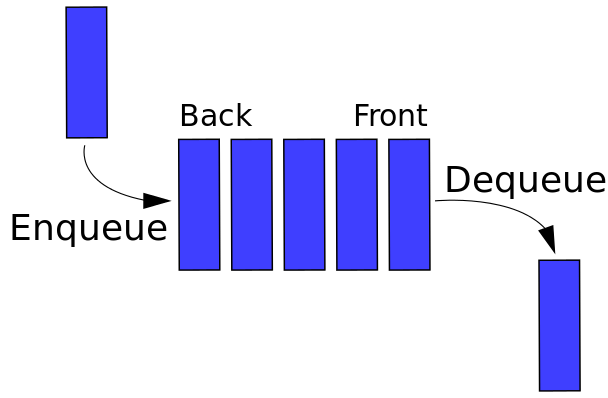
\includegraphics[width=0.7\linewidth]{queue.png}
	\caption{Representation of a FIFO (first in, first out) queue}
\end{figure}
\end{frame}

\begin{frame}
\frametitle{ FIFO }
In a FIFO data structure, the first element added to the queue will be the first one to be removed. This is equivalent to the requirement that once a new element is added, all elements that were added before have to be removed before the new element can be removed.
\end{frame} 
%--------------------------------------------------------

\section{C++ STL Queue implementation} 

\begin{frame}
\frametitle{C++ STL Queue}

\begin{block}{std::queue}
template $<$class T, class Container = deque$<$T$>$ $>$ class queue;
\end{block}

\textbf{FIFO queue}\\
queues are a type of container adaptor, specifically designed to operate in a FIFO context (first-in first-out), where elements are inserted into one end of the container and extracted from the other.

\begin{multicols}{2}
\begin{itemize}
	\item empty
	\item size
	\item front
	\item back
	\item push\_back
	\item pop\_front
\end{itemize}
\end{multicols}

The standard container classes deque and list fulfill these requirements. By default, if no container class is specified for a particular queue class instantiation, the standard container deque is used.

\end{frame}
%--------------------------------------------------------
%--------------------------------------------------------
%--------------------------------------------------------

\end{document} 
